\chapter{Experiment: the Use of Information Loss Metrics as Utility Predictors}
Although information loss metrics are widely used as proxies to measure utility, there is no evidence they are as predictive as claimed. For that reason, we propose, and carry out, an experiment to determine their use in predicting the utility of $k$-anonymous datasets on classification tasks. We $k$-anonymize the same 4 datasets with many different anonymization hyperparameters (algorithm, VGHs, choice of k), looking at overall trends, and finding out whether the information loss metrics can accurately predict utility.


\section{Overview}
The aim of this experiment is to see if information loss metrics can predict the utility of a $k$-anonymous dataset, and we break the major components into a workflow depicted in Figure \ref{fig:workflow}

\begin{figure}[h]
    \centering
    \includegraphics[width=\textwidth]{project/fig/overview.png}
    \caption{A representation of the experiment workflow. For a specific dataset, we create many different $k$-anonymous versions. For these anonymous datasets, we measure utility and the information loss metrics independently. With that information in hand, we try to make sense of it.}
    \label{fig:workflow}
\end{figure}

We start by picking four datasets that encompass a range of types of attributes and sizes. For each of these datasets, we create $600$ different $k$-anonymous versions of them, using different hyper-parameters. If information loss metrics can be used to predict utility, then, when we calculate said metrics for every anonymous dataset, and measure the datasets' utilities separately, we should be able to find some type of correlation. We use the performances of off-the-shelf classifiers trained on our anonymous datasets as a measure of utility, and avoid as much data processing on the $k$-anonymous sets as possible to remove any external influences.

Below, we explain the experimental setup for the different components involved:

\section{Datasets}
We analyze four different datasets, aiming to capture a large range of features, types, and sizes. All datasets are appropriate for classification tasks. In these datasets, the class label attribute is considered the sensitive attribute. All other attributes are quasi-identifiers.
\begin{itemize}
    \item \textbf{BIRTH} \cite{birth_dataset}: A national Indonesian survey on women’s contraceptive method of choice. It contains 1473 records and 9 quasi-identifiers, all ordinal. The sensitive attribute is the contraceptive method used (3 classes, moderately unbalanced). 
    \item \textbf{RING} \cite{ringnorm_dataset}: A synthetic dataset with points sampled from two 20-dimensional Gaussians. The first distribution has a mean of $0$ and a covariance of 4 times the identity; the second distribution has a mean of $(a,...,a)$, with $a=2/\sqrt{20}$, and a unit covariance. It contains 7400 rows and 20 continuous attributed. The sensitive attribute is the distribution from which the record was sampled (2 classes, balanced).
    \item \textbf{ADULT} \cite{adult_dataset}: Widely cited, Adult contains a slice of the results from the 1994 US Census data. Its associated classification task is predicting if an individual's salary is above or under 50k a year (our sensitive attribute). Removing records with missing entries, it contains $30,162$ rows and includes 3 ordinal, 2 continuous, and 7 unordered quasi-identifiers (2 classes, unbalanced).
    \item \textbf{HEART} \cite{heart_dataset}: A medical dataset for patients at risk of contracting a cardio vascular disease. It contains 4238 records and 15 attributes, a mix of ordinal and continuous (2 classes, heavily unbalanced).
\end{itemize}


\section{Anonymization}


\subsection{Algorithms Used}
While multiple algorithms have been proposed to achieve k-anonymity~\cite{incognito,kanon_algos,mondrian,ola_algo,arx}, we focus on two popular algorithms with an open source implementation, Datafly~\cite{kanon_algos} and Mondrian~\cite{mondrian}, using UTDallas' Anonymization Toolbox for the implementation of both algorithms \cite{utd_toolbox}. Additionally, we motivate a variant of a Datafly algorithm that removes order constraints on the attributes, thus allowing for more flexible generalization trees.

\begin{itemize}
    \item \textbf{Datafly}: For each quasi-identifier, we create a random generalization tree that respects attribute order (only adjacent attributes can be aggregated together). This variety in the generalization trees should result in datasets with differing utilities as some generalization trees will make more sense than others or preserve different pieces of information.
    
    \item \textbf{Datafly-Shuffled}: Same procedure as Datafly but removing the order constraint on the generalization tree. Intuitively, these trees ``break'' the ordinality of attibutes, and should make them less useful. Figure \ref{fig:shuffled_vgh_example} depicts an example of a possible VGH that respects order and would be used in the normal Datafly algorithm (VGH (a)), and one that could be used in a Datafly-Shuffled in which order is not respected (VGH (b)). We create this variant of Datafly to test the metrics' ability to recognise what will definitely turn into pointless anonymous datasets. We expect some metric to be unable to spot the difference, particularly those that only quantify information loss without taking into account features of the data, like Entropy.
    
    \item \textbf{Mondrian}: Mondrian assumes that all data is ordinal, and uses multi-dimensional local generalization algorithms to generalize close records together. In order to generate many random datasets, we randomly permute the values of attributes, keeping the data semantically identical but breaking the natural ordering of values. Permutations that keep a logical order are more likely to offer coherent results whereas permutations that groups values nonsensically will be less useful.
\end{itemize}

For every algorithm, we discretize continuous attributes by binning them into 20 buckets, each containing 5\% of the range of the data. When dealing with unordered attributes like Nationality, or Profession, we randomize their order, no matter the algorithm. We generate 200 $k$-anonymous versions of every dataset, for every algorithm. 


%Normal vs Shuffled VGH
\begin{figure}
\centering
\subfigure[VGH, respecting order]{
    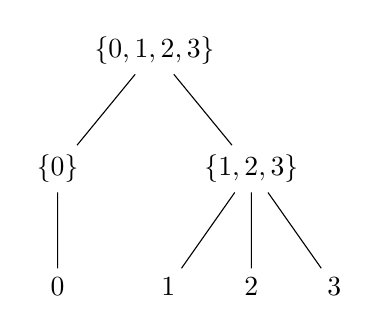
\begin{tikzpicture}[sibling distance=7em,
    level 2/.style={sibling distance=3em}]]
    \node {$\{0,1,2,3\}$} 
        child { node {$\{0\}$}
            child { node {$0$}}
        }
        child { node {$\{1,2,3\}$}
            child { node {$1$}}
            child { node {$2$}}
            child { node {$3$}}
        }
    ;
    \end{tikzpicture}}
\hspace{2cm}
\subfigure[VGH, unordered]{
    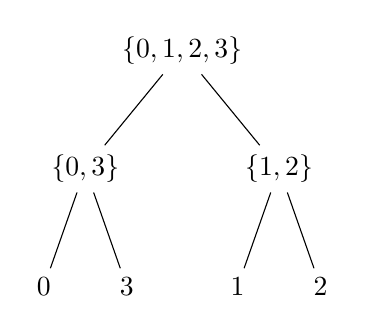
\begin{tikzpicture}[sibling distance=7em,
    level 2/.style={sibling distance=3em}]]
    \node {$\{0,1,2,3\}$} 
        child { node {$\{0,3\}$}
            child { node {$0$}}
            child { node {$3$}}
        }
        child { node {$\{1,2\}$}
            child { node {$1$}}
            child { node {$2$}}
        }
    ;
    \end{tikzpicture}}
\caption{Two example of possible VGHs on a categorical attribute with 4 possible values. The left-hand-side VGH respects order; the right-hand-side VGH does not}
\label{fig:shuffled_vgh_example}
\end{figure}


\subsection{VGH Creation}
To create random VGHs, we use sets to represent the generalization levels. For example, a cell with value $\{0,1,2,3\}$ could have any of the elements in the set as an original value.

The procedure is as follows:
\begin{enumerate}
    \item We start with a full set of the domain ground values. This represents the fully suppressed value at the top of the generalization tree.
    \item We split this set into an ordered partition-- a partition in which values still appear in increasing order.
    \item We recursively keep on splitting the subsets of the partitions, until we reach a singleton elements, representing the ground domain values. 
\end{enumerate}

This returns a tree of values, with ground values as leaves, with a generalization for every step up the tree. However, we have an additional constraint: every leaf node needs to be at the same depth. This is because Datafly performs global single-dimensional generalizations and we thus need coherence between the generalization levels of values within an attribute. As such, we find the shallowest leaf node in our tree, and prune any branch that extends past that by setting all the elements in the parent node as individual leaves. Figure \ref{fig:vgh_creation} displays an example of a possible generalization tree creation before we insert the depth constraint, and after. 

\begin{figure}
\centering
\subfigure[VGH, no depth constraint]{
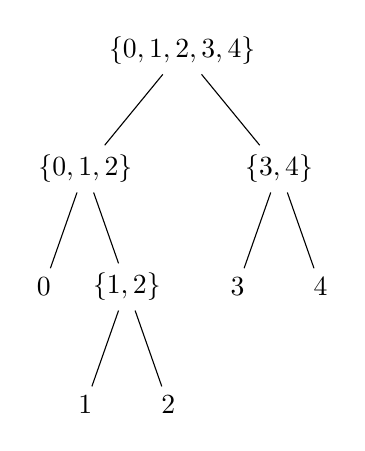
\begin{tikzpicture}[sibling distance=7em,
    level 2/.style={sibling distance=3em},
    level 3/.style={sibling distance=3em}]]
    \node {$\{0,1,2,3,4\}$} 
        child { node {$\{0,1,2\}$}
            child { node {$0$}}
            child { node {\{$1,2$\}}
                child {node {$1$}}
                child {node {$2$}}
            }
        }
        child { node {$\{3,4\}$}
            child { node {$3$}}
            child { node {$4$}}
        }
    ;
    \end{tikzpicture}}
\hspace{2cm}
\subfigure[VGH, with depth constraint]{
    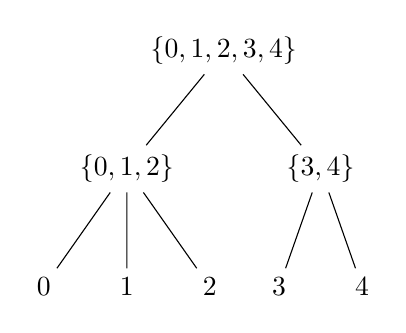
\begin{tikzpicture}[sibling distance=7em,
    level 2/.style={sibling distance=3em},
    level 3/.style={sibling distance=3em}]]
    \node {$\{0,1,2,3,4\}$} 
        child { node {$\{0,1,2\}$}
            child { node {$0$}}
            child { node {$1$}}
            child { node {$2$}}
        }
        child { node {$\{3,4\}$}
            child { node {$3$}}
            child { node {$4$}}
        }
    ;
    \end{tikzpicture}}
\caption{An example of how a generalization tree randomly created for a 5-valued attribute, and how that tree looks when respecting the depth constraint. The shallowest leaf in VGH (a) occurs at depth 2 so we turn the set $\{1,2\}$ into two separate leaves, and prune any branch extending deeper}
\label{fig:vgh_creation}
\end{figure}

\subsection{Choice of k}
An initial exploration revealed that an increasing $k$ value quickly destroyed the dataset, and, ultimately, led to noisy, nearly random classification results, with very little utility for a classification task. We show this in Figure \ref{fig:varying_k_birth_mondrian_knn} for a Mondrian algorithm on the Birth dataset using a k-Nearest Neighbour Classifier. We see a slight decreasing trend in utility until around the $k=20$ mark, after which the results, become very noisy but seem to have very little utility, as judged by the dashed black line representing the accuracy baseline.

\begin{figure}
    \centerfloat
    \includegraphics[width=1.2\textwidth]{project/fig/varying_k_birth_mondrian_knn.png}
    \caption{Plot of the measured accuracy (blue) and a baseline accuracy for a k-Nearest Neighbour Classifier trained on a Mondrian $k$-anonymous birth dataset with increasing $k$ values. The dashed black line represents the accuracy baseline. The results show an initial steep decrease in accuracy (i.e., utility) that flattens out quickly. For values larger than $k=20$, we assume the varying results are noise.}
    \label{fig:varying_k_birth_mondrian_knn}
\end{figure}

Because the most significant data destruction happens for small values of $k$, we restrict our $k$ parameter choice to small values. Nevertheless, we found that fixing $k=2$ could restrict the range of some metrics. In an attempt to add some flexibility, we set the k parameters of the 200 datasets to samples from $k = X + 2$, where $X \sim Poi(1)$. This guarantees small $k \geq 2$ values, but also grants a larger range for the information loss metrics.

\section{Machine Learning Tasks}
\subsection{Pre-Processing Anonymous Datasets}
After the anonymization, we need a way to format the results so we can use them in our classification tasks. They cannot be left as a single range per attribute because there are unordered shuffled attributes that could potentially lead to disjoint sets of possible original values. We choose a solution akin to one-hotting: we turn every record into binary tuples of possible original values. Take a cell $x_{ij}$ from an anonymous record, representing a set of values. For the set of values in attribute $A_j$, $\{a_j^{(1)},...,a_j^{(l)}\}$, we turn anonymous cell $x_{ij}$ into a binary tuple of size $l$, defined as follows: 

$$t_{ij} = (1 \mbox{ if } a_j^{(k)} \in x_{ij} \mbox{ else } 0)_{k=1}^l$$

We rebuild records by concatenating the tuples for all attributes.

As an example, take the dataset with attributes Age, categorically ranging from $0$ to $3$, and Gender, a binary choice, in Table \ref{tab:bitmap_example}. This method allows for arbitrary sets of numbers, and can thus be used for all our algorithms.

\begin{figure}
\centering
\subfigure[$D'$, a $2$-anonymous dataset]{
    \begin{tabular}{|l|l|}
        \hline
        Gender & Age \\
        \hline
        \{0\} & \{1,3\}  \\
        \{0\} & \{1,3\}  \\
        \{0, 1\} & \{0,1\}  \\
        \{0, 1\} & \{0,1\}  \\
        \hline
    \end{tabular}}
\subfigure[D', as a concatenation of tuples]{
\begin{tabular}{|l|l|l|l|l|l|}
\hline
gender\_0 & gender\_1 & age\_0 & age\_1 & age\_2 & age\_3\\
\hline
1 & 0 & 0 & 1 & 0 & 1 \\
1 & 0 & 0 & 1 & 0 & 1 \\
1 & 1 & 1 & 1 & 0 & 0 \\
1 & 1 & 1 & 1 & 0 & 0 \\
\hline
\end{tabular}}
\caption{An example to show a transformation between cells containing sets of values for age and gender attributes into binary tuples representing the same information}
\label{tab:bitmap_example}
\end{figure}

We apply the same process to the original data, essentially one-hotting it.

\subsection{Classifiers and Utility Measures}
\label{sec:util_measures}
For this project, we use our $k$-anonymous datasets as training sets for off-the-shelf classifiers and test their performance on the original test data. We equate a dataset's utility to the obtained performances when used as a training set.

To reduce the risk of measuring metric utilities that will be entirely dependent on the classifier used, we train three types of classifiers for every dataset, and measure both accuracy, and the Area Under the Receiver operating characteristic (AUROC). The three types of classifiers are as follow: 

\begin{itemize}
    \item Logistic Regression
    \item Random Forest after Principal Component Analysis (PCA) transformation with .95 explained variance
    \item K-Nearest Neighbours after PCA transformation with .95 explained variance
\end{itemize}
Although the idea was to keep the anonymous data manipulation to a strict minimum, avoiding any external factors that could affect measured utility, the number of columns after turning records into binary arrays was such that the Curse of Dimensionality became an issue. Therefore, we add a PCA transformation to the two classifiers most sensitive to this problem. Additionally, the datasets were so destroyed by the anonymization process-- most columns would be fully suppressed--  that an explained variance of $0.95$ could usually be reached in very few dimensions, making k-NN and RF classifiers simple and intuitive choices.

This method of measuring utility results in 600 different $k$-anonymous versions of every dataset (200 for each algorithm used), with six different measures of utility.



\section{Metrics Used}
We implement all the metrics described in the Information Loss Metrics section (\ref{sec:metrics}) apart from Precision. This is because the metric takes into account the anonymous dataset's DGHs' depths and would require us to extend the definition of this metric for the Mondrian anonymizations, in which the concept of depth is inapplicable. To keep the experiment constant over all the algorithms, we decide to forego Precision.

These metrics were chosen because they were either presented with the purpose of measuring utility, or because they have been used as utility predictors in the literature and/or industry.

We design our experiment to scale every metric into the range $[0,1]$. Some metrics occur in this range by definition, like the Classification Metric. For the others, we divide the result by the worse possible case metric: we take a fully suppressed version of the dataset, and calculate the metric of that dataset.


\section{Meta-Metric}
\label{sec:metametrics}
The results, found in Chapter \ref{chap:results}, imply very little correlation between information loss metrics and dataset utility. Nevertheless, we do not reach a definite conclusion because the claim that metrics reflect utility is difficulty falsifiable-- the metrics might very well reflect utility except that we simply do not understand how to use them correctly. 

Instead, we propose a secondary analysis: if, when given all the metrics, we can train a regressive model that correctly predicts utility in datasets, then the metrics must have some predictive power. Here, we try to emulate the best case situation: our model will learn as much information as it can on all the combined metrics and the resulting measured utilities, and will therefore be able to make much deeper inferences than we could. Therefore, if the model can predict utility, then we must concede that somewhere in the metrics lies information about utility and that we just could not see it. However, if the model still cannot predict utility, then it must be that the metrics are not viable because even a model trained on the task could not draw the link between them.

We design our Regression model to take a dataset in which the features are our metrics, and every row represents a $k$-anonymous dataset on which we calculated the metrics. The target variable for a model will be one of the different utility measures we describe in Section \ref{sec:util_measures}. For every model, we take 10\% of our data as a testing set.

We use a library called auto-sklearn, an automated machine learning toolkit \cite{autosklearn}. Given a single parameter, running time, this library uses Bayesian optimization and meta-learning to construct an ensemble model for a regression task. This allows us to train regressors on our metrics impartially by giving each learning task the same amount of time to train: 24 hours. The resulting ensemble will be our best predictor at the potential accuracy of our test datasets and we coin it a Meta-Metric. 

We train an auto-sklearn model per utility measure, and per dataset. Furthermore, we need to separate the algorithms used. This is because, as seen in the scatterplots \ref{fig:metrics_scatter1} and \ref{fig:metrics_scatter2}, the metric results for Datafly algorithms are disjoint clusters from the Mondrian results (we explain further in Section \ref{sec:single_metrics}). This is a problem as any decent machine-learning task can distinguish between two separate clusters. Additionally, we know that Mondrian datasets tend to outperform Datafly datasets in the utility measures. Because of those disparities in both the utility measures, and the metrics, our model would only have to learn to differentiate between a Mondrian and Datafly algorithm to score well. However, this simplifies the task, and the algorithm used should be irrelevant. As such, the model will be a better predictor of utility than it should be because, instead of predicting the utility of the metrics, it will predict whether the dataset will have the utility of a Mondrian dataset, or a Datafly one.






